\section{Pruebas de bondad de ajuste}

\begin{frame}{Pruebas de bondad de ajuste}
    \begin{itemize}
        \item Las pruebas de bondad de ajuste son pruebas de hipótesis para verificar si los datos observados en una muestra aleatoria se ajustan con algún nivel de significancia a determinada distribución de probabilidad.
        \item Las hipótesis son:
        \begin{itemize}
            \item $H_0$: la variable aleatoria $X$ sigue una distribución asumida con los parámetros estimados.
            \item $H_1$: la variable aleatoria $X$ no sigue la distribución asumida.
        \end{itemize}
        \item Para realizar la prueba, se clasifican los datos observados en $k$ clases y se contabiliza el número de observaciones en cada clase, posteriormente se compara la frecuencia observada en cada clase con la frecuencia esperada en esa clase si la hipótesis nula es correcta.
    \end{itemize}
\end{frame}

\begin{frame}{Prueba chi-cuadrado}
    \begin{itemize}
        \item Considere $k>2$ el núméro de clases, $O_i$ la frecuencia observada en la clase $i$, $E_i$ la frecuencia esperada en la clase $i$ si $H_0$ es correcta.
        \item La prueba se basa en el estadístico de prueba chi-cuadrado:
        \[Y=\sum_{i=1}^{k}{\frac{\left(O_i-E_i\right)^2}{E_i}}\]
        \item El estadístico sigue una distribución chi-cuadrado con $k-r-1$ grados de libertad, donde $r$ es el número de parámetros estimados en $f_0(x)$ para encontrar $E_i$. 
    \end{itemize}
\end{frame}


\begin{frame}{Prueba chi-cuadrado}{Consideraciones}
    \begin{itemize}
        \item Si las diferencias $O_i-E_i$ son pequeñas, el valor del estadístico es pequeño, por el contrario si esas diferencias son grandes el valor del estadístico es grande.
        \item El tamaño de la muestra deberá ser moderadamente grande, pues si la muestra es muy pequeña no se podrá formar un número suficiente de clases y si la muestra es muy grande la prueba conducirá a rechazo casi con seguridad. 
        \item Se sugiere evitar tener clases con $E_i$ menores que 5, esto puede conseguirse combinando clases vecinas. Tenga en cuenta que para calcular los grados de libertad, $k$ es el número de clases efectivas.
    \end{itemize}
\end{frame}

\begin{frame}{Prueba chi-cuadrado}
    \begin{figure}
        \centering
        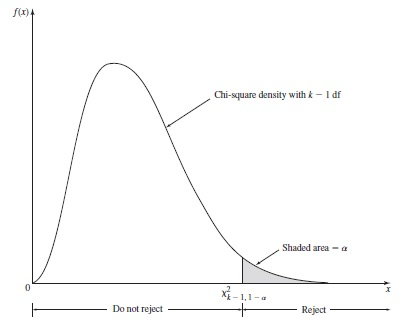
\includegraphics[width=8cm]{images/Chi-square.jpg}
        %\caption{Caption}
        \label{fig:chisquare}
    \end{figure}
\end{frame}
\begin{frame}{Prueba de Kolmogorov-Smirnov}
    \begin{itemize}
        \item Esta prueba formaliza la idea de una gráfica cuantil-cuantil y compara una función empírica de probabilidad con la función de la distribución hipotética. 
        \item No requiere de especificación de intervalos y es válida para cualquier tamaño de muestra.
    \end{itemize}
\end{frame}

\begin{frame}{Prueba de Kolmogorov-Smirnov}{Algoritmo}
    \begin{enumerate}
        \item Tomar una muestra de los datos $x_i,~i=1,2,\dots,n$ y ordenarlos para obtener $y_j,~j=1,2,\dots,n$.
        \item Estimar las diferencias por arriba y por abajo: $D^+=\max \left[ \frac{j}{n}-F(y_j)\right]$ y $D^-=\max \left[ F(y_j)-\frac{j-1}{n}\right]$. El estadístico de prueba está dado por: $D:\max \left[D^+,D^-\right]$
        \item Determine el valor crítico $D_\alpha$ para un nivel de significancia $\alpha$ y un tamaño de muestra $N$.
        \item Si el estadístico calculado es mayor que el valor crítico, entonces se rechaza la hipótesis nula. De lo contrario, se concluye que no hay evidencia estadística para recharzarla.
    \end{enumerate}
\end{frame}

\begin{frame}{Prueba de Kolmogorov-Smirnov}
\begin{figure}
    \centering
    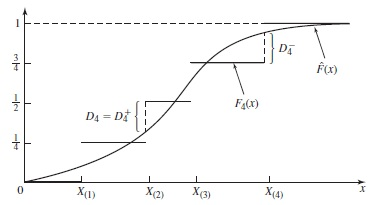
\includegraphics[width=8cm]{images/kolmogorov.jpg}
    %\caption{Caption}
    \label{fig:kolmogorov}
\end{figure}
\end{frame}

\begin{frame}{p-value}
    \begin{itemize}
        \item El p-value es el nivel de significancia en el que se rechazaría $H_0$ para el valor dado del estadístico de prueba. Por lo tanto, un p-value alto tiende a indicar un buen ajuste (tendríamos que aceptar una gran posibilidad de error para rechazar), mientras que un p-value pequeño sugiere un mal ajuste.
        \item El p-value se puede ver como una medida de ajuste, siendo mejores los valores más grandes. Regla de rechazo: si el p-value es menor que el nivel de significancia entonces se debe rechazar la hipótesis nula.
    \end{itemize}
\end{frame}